\section{Presentación de resultados}

\subsection{Práctica 1}

\subsubsection{Puntos de operación}

En el cuadro \ref{tab:med-puntos-dc-etapa-potencia} se muestran las mediciones DC de las transistores Q4, Q5 y Q6 necesarios para obtener los puntos de operación en la etapa de potencia. 

\begin{table}[ht]
\centering
\begin{tabular}{|c|c|c|c|c|c|c|c|c|c|c|}
\hline
\textbf{Transistor} & \textbf{Vc()} & \textbf{$\varDelta$ Vc()} & \textbf{Vb()} & \textbf{$\varDelta$ Vb()} & \textbf{Ve()} & \textbf{$\varDelta$ Ve()} & \textbf{Ve2} & \textbf{$\varDelta$ Ve2} & \textbf{Re} & \textbf{$\varDelta$ Re2} \\ \hline
Q4 & 0.7 & 0.01 & 0 & 0.01 & -0.6 & 0.004 & 5000 & 500 & 20 & 1 \\
\hline
Q5 & 10 & 1 & 0.7 & 0.1 & 0.05 & 0.01 & 0.02 & 0.004 & 20 & 1 \\ \hline
Q6 & -10 & 1 & -0.56 & 0.04 & 0.02 & 0.004 & 0.05 & 0.01 & 20 & 1 \\ \hline
\end{tabular}
\caption{Mediciones DC etapa de potencia}
\label{tab:med-puntos-dc-etapa-potencia}
\end{table}

Usando las mediciones del cuadro \ref{tab:med-puntos-dc-etapa-potencia} se calculan los puntos de operación en la etapa de potencia representados en los cuadros \ref{tab:ic-practica-1} y \ref{tab:med-voltajes_ce_etapa_potencia}.

\begin{table}[ht]
\centering
\begin{tabular}{|c|c|c|c|c|c|}
\hline
Transistor & Teórico & Medición & Incertidumbre & Error Absoluto & Error Relativo \\\hline
Q4 & $302.36 \times 10^{-6}$ & $120 \times 10^{-6}$ & $12.1918 \times 10^{-6}$ & $182.36 \times 10^{-6}$ & 60\% \\\hline
Q5 & $350 \times 10^{-6}$ & $1.50 \times 10^{-3}$ & $543.714 \times 10^{-6}$ & $1.150 \times 10^{-3}$ & 329\% \\\hline
Q6 & $350 \times 10^{-6}$ & $-1.50 \times 10^{-3}$ & $543.714 \times 10^{-6}$ & $1.850 \times 10^{-3}$ & 529\% \\\hline
\end{tabular}
\caption{Corrientes colector práctica 1}
\label{tab:ic-practica-1}
\end{table}

\begin{table}[h!]
\centering
\begin{tabular}{|c|c|c|c|c|c|}
\hline
\textbf{Transistor} & \textbf{\(Vce [V]\)} & \textbf{Medición} & \textbf{Incertidumbre} & \textbf{Error Absoluto} & \textbf{Error Relativo} \\ \hline
Q4 & 1.24 & 1.30000000000000 & 0.01077033 & 0.06000000 & 4.84\% \\ \hline
Q5 & 9.99 & 9.95000000000000 & 1.000049999 & 0.04000000 & 0.40\% \\ \hline
Q6 & -9.99 & -10.0200000000000 & 1.000008 & 0.03000000 & -0.30\% \\ \hline
\end{tabular}
\caption{Voltajes \(V_{ce}\) de la etapa de potencia}
\label{tab:med-voltajes_ce_etapa_potencia}
\end{table}


\subsubsection{Modelo dinámico}

El cuadro \ref{tab:med-impedancia_entrada-etapa-potencia} muestra los datos para calcular la impedancia de entrada en la etapa de potencia.

\begin{table}[h!]
\centering
\begin{tabular}{|c|c|c|c|c|c|}
\hline
\textbf{\(Vg[V]\)} & \textbf{\(\varDelta Vg[V]\)} & \textbf{\(Vi[V]\)} & \textbf{\(\varDelta Vi[V]\)} & \textbf{\(Rp[\Omega]\)} & \textbf{\(\varDelta Rp[\Omega]\)} \\ \hline
0.52 & 0.04 & 0.26 & 0.02 & 10000 & 100 \\ \hline
\end{tabular}
\caption{Mediciones para calcular impedancia de entrada en la etapa de potencia}
\label{tab:med-impedancia_entrada-etapa-potencia}
\end{table}

El cuadro \ref{tab:med-impedancia_salida-etapa-potencia} muestra los datos para calcular la impedancia de salida en la etapa de potencia.

\begin{table}[h!]
\centering
\begin{tabular}{|c|c|c|c|c|c|}
\hline
\textbf{\(Vo_{sc}[V]\)} & \textbf{\(\varDelta Vo_{sc}[V]\)} & \textbf{\(Vo_{cc}[V]\)} & \textbf{\(\varDelta Vo_{cc}[V]\)} & \textbf{\(Rp[\Omega]\)} & \textbf{\(\varDelta Rp[\Omega]\)} \\ \hline
0.52 & 0.05 & 0.24 & 0.02 & 10 & 1 \\ \hline
\end{tabular}
\caption{Mediciones para calcular la impedancia de salida en la etapa de potencia}
\label{tab:med-impedancia_salida-etapa-potencia}
\end{table}



El cuadro \ref{tab:entrada_salida_etapa_potencia} muestra los datos de voltaje de entrada y salida en la etapa de potencia.

\begin{table}[h!]
\centering
\begin{tabular}{|c|c|c|c|}
\hline
\textbf{\(Vi[V]\)} & \textbf{\(\varDelta Vi[V]\)} & \textbf{\(Vo[V]\)} & \textbf{\(\varDelta Vo[V]\)} \\ \hline
0.52 & 0.04 & 0.48 & 0.04 \\ \hline
\end{tabular}
\caption{Datos de voltaje de entrada y salida etapa de potencia}
\label{tab:entrada_salida_etapa_potencia}
\end{table}

Usando los datos medidos en los cuadros \ref{tab:entrada_salida_etapa_potencia}, \ref{tab:med-impedancia_entrada-etapa-potencia} y \ref{tab:med-impedancia_salida-etapa-potencia} se calculan los valores de los parámetros del modelo dinámico de la etapa de potencia representados en el cuadro \ref{tab:med-modelo-dinamico-etapa-potencia}.

\begin{table}[ht]
\centering
\begin{tabular}{|c|c|c|c|c|c|}
\hline
\textbf{Parámetro} & \textbf{Valor Teórico} & \textbf{Medición} & \textbf{Incertidumbre} & \textbf{Error Absoluto} & \textbf{Error Relativo} \\ \hline
$Z_i[O]$ & 10770 & 10000 & 2178.010058 & 770.00000000 & 7.15\% \\ \hline
$Z_o[O]$ & 132 & 11.66666667 & 2.993563053 & 120.33333333 & 91.16\% \\ \hline
$A$ & 0.96 & 0.923076923 & 0.104685243 & 0.03692308 & 3.85\% \\ \hline
\end{tabular}
\caption{Mediciones modelo dinámico etapa de potencia}
\label{tab:med-modelo-dinamico-etapa-potencia}
\end{table}

\subsubsection{Transistor clase C}

En el cuadro \ref{tab:med-dc-etapa-potencia-clase-c} se muestran las mediciones DC
de operación en la etapa de potencia conectado como amplificador clase C.

\begin{table}[h!]
\centering
\begin{tabular}{|c|c|c|c|c|c|c|c|c|}
\hline
\textbf{Transistor} & \textbf{\(Vc[V]\)} & \textbf{\(\varDelta Vc[V]\)} & \textbf{\(Vb[V]\)} & \textbf{\(\varDelta Vb[V]\)} & \textbf{\(Ve[V]\)} & \textbf{\(\varDelta Ve[V]\)} & \textbf{\(Re[\Omega]\)} & \textbf{\(\varDelta Re[\Omega]\)} \\ \hline
Q4 & 0.7 & 0.01 & 0 & 0.01 & -0.6 & 0.004 & 5000 & 500 \\ \hline
Q5 & 10 & 1 & 0.4 & 0.0004 & -0.04 & 0.02 & 20 & 1 \\ \hline
Q6 & -10 & 1 & -0.34 & 0.02 & -0.026 & 0.004 & 20 & 1 \\ \hline
\end{tabular}
\caption{Mediciones DC etapa de potencia clase C}
\label{tab:med-dc-etapa-potencia-clase-c}
\end{table}

Con el cuadro \ref{tab:med-dc-etapa-potencia-clase-c} se muestran los puntos de operación en la etapa de potencia conectado como amplificador clase C de la figura \ref{tab:med-punto-estatico-etapa-potencia-clase-c}.

\begin{table}[h!]
\centering
\begin{tabular}{|c|c|c|c|c|c|c|}
\hline
\textbf{Transistor} & \textbf{Parámetro} & \textbf{Valor Teórico} & \textbf{Medición} & \textbf{Incertidumbre} & \textbf{Error Absoluto} & \textbf{Error Relativo} \\ \hline
Q4 & \(Ic [A]\) & 3.02E-04 & 0.00012 & 1.21918E-05 & 0.00018236 & 60.31\% \\ \hline
Q5 & \(Ic [A]\) & 3.50E-04 & -0.0007 & 0.001020404 & 0.00105000 & 300.00\% \\ \hline
Q6 & \(Ic [A]\) & 3.50E-04 & 0.0007 & 0.001020404 & 0.00035000 & 100.00\% \\ \hline
Q4 & \(Vce [V]\) & 1.24 & 1.3 & 0.01077033 & 0.06000000 & 4.84\% \\ \hline
Q5 & \(Vce [V]\) & 9.99 & 10.04 & 1.00019998 & 0.05000000 & 0.50\% \\ \hline
Q6 & \(Vce [V]\) & -9.99 & -9.974 & 1.000008 & 0.01600000 & -0.16\% \\ \hline
\end{tabular}
\caption{Voltajes \(V_{ce}\) de la etapa de potencia}
\label{tab:med-punto-estatico-etapa-potencia-clase-c}
\end{table}

En la figura \ref{fig:efecto-crossover-amplificador-clase-c} se muestra el efecto crossover del amplificador clase C de la etapa de potencia.

\begin{figure}
    \centering
    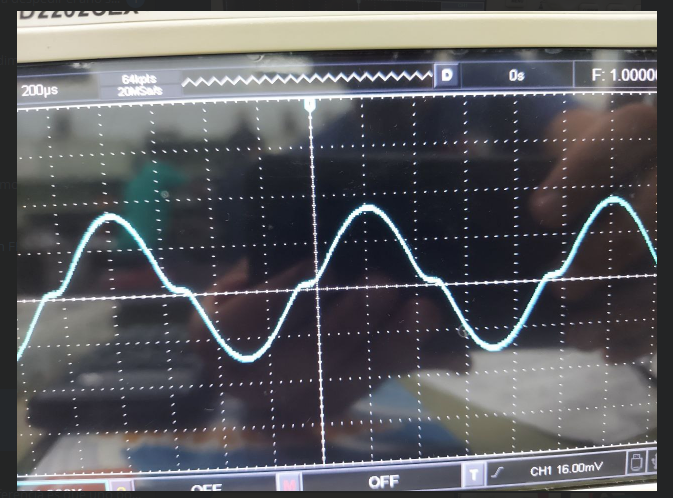
\includegraphics[width=0.8\textwidth]{src/images/p1/p1-efecto-crossover.png}
    \caption{Efecto crossover amplificador clase C de la etapa de potencia}
    \label{fig:efecto-crossover-amplificador-clase-c}
\end{figure}
